\documentclass{scrartcl}
\usepackage[utf8]{inputenc}
\usepackage{graphicx}
\usepackage{subfigure}
\usepackage{supertabular}
\usepackage{float}
\usepackage{booktabs, tabularx}
\begin{document}

\title{Documentation for the RAxML EPA Webserver}
\author{Denis Krompass\\ dekromp@googlemail.com}
\maketitle

\tableofcontents
	%%%%%%%%%%%%%%%%%%%%%%%%%%%%%%%%%%%%%%%%%%%%%%%%%%%%%%%%%%%%%%%%%
	%%%% APPLICATION CONCEPT & STRUCTURE
	\section{Application concept \& structure }
		The Web-Interface for the RAxML Evolutionary Placement Algorithm is written in Ruby using the Ruby on Rails Framework for web-applications. I recommend reading the first chapters of a Ruby on Rails book (e.g. Agile web development with Rails) or at least an online tutorial to understand the basic ideas and concepts of  the framework. There is some "magic" happening in the background of a Rails application that cannot be seen within the scripts and programs that are described here. So somebody who has no idea about these functionalities provided by the framework might get confused about how this collection of scripts can actually work when looking solely at the code.  \\
		In this documentation I will try to explain how the scripts and programs are connected  and work together. Besides that I will try to give an overview of the jobs each script fulfils to ease debugging or developing new functions within the application in the future. However, I will not provide any explanations to any programming details here. The details can be discovered directly by looking at the code. Some words about my code and programming style respectively. I always try to use meaningful names for variables, methods and classes that explain their content or their functionality. Therefore I often resign using comments where in my opinion the naming is enough for the  understanding. An overview of the concept of the web-application is given in figure \ref{fig:concept}. In the following sections this concept will be explained. Starting by the views and digging from there deeper into the application.
		
	%%%% CONCEPT FIGURE			
		\begin{figure}[htb]
		\centering
		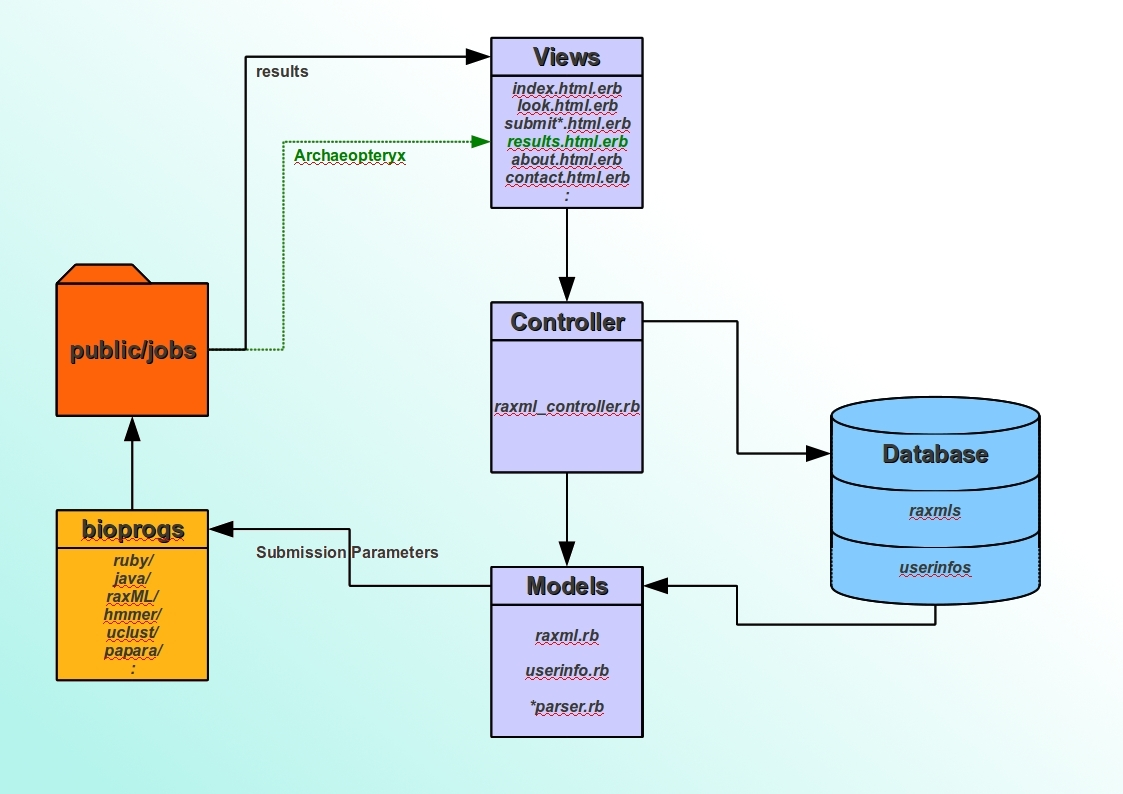
\includegraphics[scale=0.30]{./RAxMLWS_Concept}
		\caption{The basic concept and structure of the RAxML-EPA Webinterface}
		\label{fig:concept}
		\end{figure}		
		
		%%%%%%%%%%%%%%%%%%%%%%%%%%%%%%%%%%%%%%%%%%%%%%%%%%%%%%%%%%%%%%%%%%%
		%%%% FOLDER HIERARCHY
		\subsection{The folder hierarchy}	
			In this section I will talk a little bit about the structure of the application.
			When looking in the root directory of the Rails-Application (\texttt{RAxMLWS/}), there are a couple important folders: \\
			\begin{tabular}[c]{lp{12cm}l}
			\texttt{app} &  This folder contains all the models, views and the controller  scripts used. The details of these files will be discussed in the next sections. \\
				\texttt{bioprogs} & This is an "artificial" folder not provided by the default rails framework. It contains different helper scripts and programs (e.g. RAxML) used by the web-application. \\
				\texttt{config} & The rails configurations. Some relevant details are also discussed in a later section. \\
				\texttt{db} &	Here are the database details provided. Unfortunately rake db::migrate does not work when altering the models and tables that are already present in the database. This has to be done manually by hand in SQL.  \\
				\texttt{log} & All the rails logs are stored here. \\
				\texttt{public} & The public folder contains all kinds of stuff including things the Apache can access like the Archaeopteryx applet and images, and also JavaScript-Scripts and Stylesheets used by the views. This folder also contains Job folders from the users including the job specific results and input files. \\
				\texttt{test} & The application has a test-routine that tests some use-cases. Testing is covered in the "Testing" section. \\
				\texttt{testfiles} & This folder contains test-files that simulate use-cases for the test-routine. \\
			\end{tabular}
		
		
		%%%%%%%%%%%%%%%%%%%%%%%%%%%%%%%%%%%%%%%%%%%%%%%%%
		%%%% VIEWS 
		\subsection{Views}
			Views are the user-interaction-interfaces of the web-application. In this case html.erb pages ("erb" is a synonym for "embedded ruby"). All the views have a common layout which is defined by  \texttt{app/views/layouts/raxml.html.erb}. The navigation bar (figure \ref{fig:views} green) is defined by \texttt{app/views/shared/\_navigation.html.erb}. The content (figure \ref{fig:views} blue area) is variable and defined by the views stored in \texttt{app/views/raxml/}. In most of the cases the views only define the structure of the web-page. The appearance and some extra functionality is defined by an external CSS-Stylesheet (\texttt{raxml.css}) and an external JavaScript script (\texttt{application.js}). These files can be found  in \texttt{public/stylesheets/} or \texttt{public/javascripts/} respectively. 
			
		%%%% VIEWS FIGURE
		\begin{figure}[htb]
		\centering
		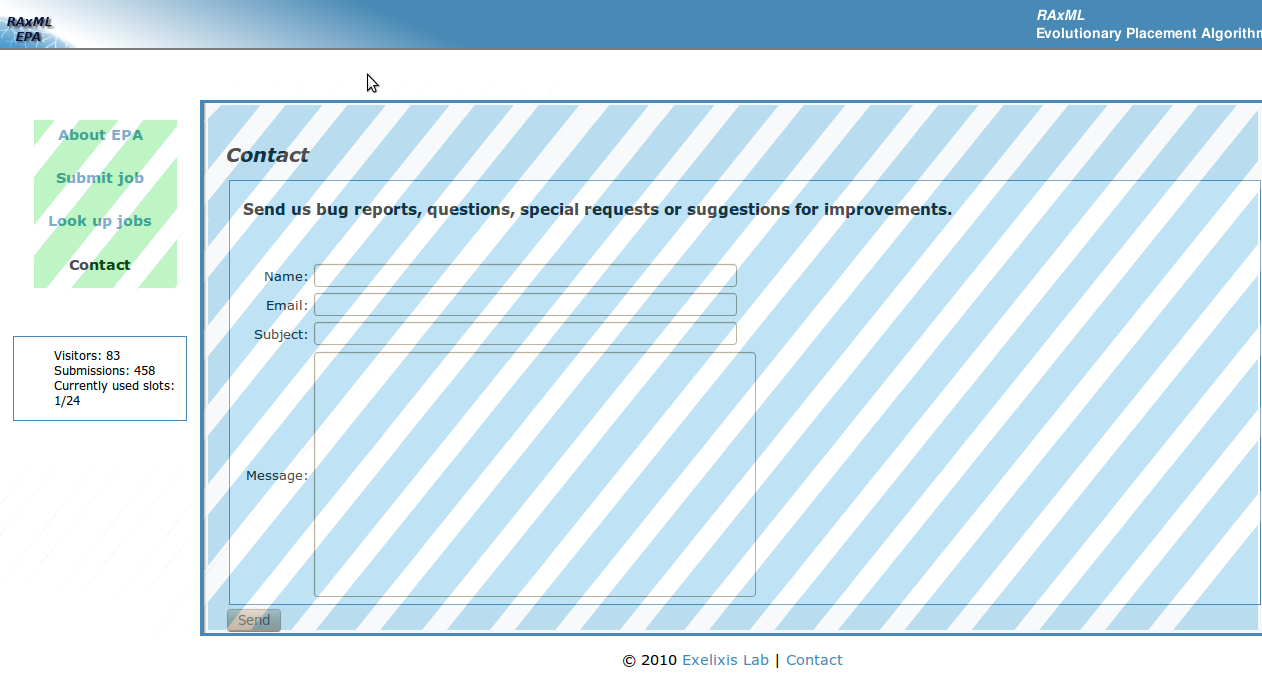
\includegraphics[scale=0.30]{./views}
		\caption{The Webpage Layout}
		\label{fig:views}
		\end{figure}
		
		%%%%%%%%%%%%%%%%%%%%%%%%%%%%%%%%%%%%%%%%%%%%%%%%%%
		%%%% CONTROLLERS
		\subsection{Controllers}
		As denoted by their name, controllers control the actions performed within the view. Basically all views in  \texttt{app/views/raxml/} have a method with the same name defined in the controller, which is executed before the associated view is interpreted. This is useful when you need to display data from an external source within the view (e.g. from a MySQL database). Rails allows you to define global variables within the controller methods that can be accessed within the view. For instance if you want to list all jobIDs for a certain user in your \texttt{yourExamplePage.html.erb} , you can do so by loading the desired data within a controller method called   \texttt{yourExamplePage} from the database and save it in a global variable (marked by an @, e.g. @jobIDs). It is then possible to read this variable within the view using embedded ruby (denoted by the "\texttt{$<$\%= @jobIDs \%$>$}  tags. The \texttt{allJobs.html.erb} view is a concrete example for this  procedure. \\
		 It is also possible to define custom methods for fired actions in a view (e.g. pressing the submit button), that are not associated with a view by themselves. The \texttt{submitJob} method for instance is only controlling but has no own view associated with it. This method only collects the input parameters from a view, validates them, saves them in the database, executes the follow up programs and redirects the user to the waiting view.
		 
		%%%%%%%%%%%%%%%%%%%%%%%%%%%%%%%%%%%%%%%%%%%%%%%%%%%%%%%%%%%%%%%%%
		%%%% Models and the database
		\subsection{Models and the database}
			Models in rails are objects first of all. The difference  to "ordinary" objects lies in the fact, that Rails models are directly associated to the database tables. In case of the model \textit{raxml} exists a table \textit{raxmls} in the database \textit{RAxMLWS\_development} that represents the model on database level. The columns contain the attributes and their values, where each row represents one  instance of the model. When accessing and manipulating an instance of a model it is possible to manipulate the associated table entries without using SQL queries within the code. The concrete case of this rails application, there are only  two models present. The \textit{raxml} model (\texttt{raxml.rb}) that holds the submission parameters  for  the EPA and performs the validation of those. It also builds a shell script to submit the job to the grid. The second model \textit{userinfo} (\texttt{userinfo.rb}) holds  the user informations like IP and email address for statistical and job mapping purposes. The detailed table infos for the two models are displayed in table \ref{tab:raxmls} and table \ref{tab:userinfos}. Observe that there is no declaration of attributes in the ruby scripts belonging to the model. The model knows its attributes solely from the table definition within the database. \\
			The database-rails-interaction is basically configured by two different files. On the one side there is the connection file \texttt{config/database.yml} which contains the connection parameters to the database. On the other side there is the schema file \texttt{db/schema.rb}  which holds the table definitions.
			
		%%%% RAXMLS TABLE
		\begin{table}[]
			\caption{raxmls table}
			\label{tab:raxmls}
			\begin{tabular}[c]{l|l}
				\hline \textbf{raxmls attributes} & \textbf{description} \\	
				\hline id & The default primary key \\
				query & The alignment type\\
				alifile & Path of the alignment file on the hard drive\\
				treefile & Path of the treefile on the hard drive \\
				outfile & Obsolete relict\\
				substmodel & The substitution model used e.g. GTRGAMMA \\
				speed  &  \texttt{T} or \texttt{F} for using a faster algorithm\\
				heuristic & \texttt{MP} or \texttt{ML}\\
				h\_value & Heuristic value\\
				email & User email address \\
				errorfile & Path of the SGE error file on the hard drive\\
				parfile & Path of the partition-file on the hard drive\\ 
				queryfile & Path of the queryreads-file on the hard drive\\
				jobid & The unique jobid\\
				user\_ip & User IP address\\
				job\_description & User specific job description\\
				b\_random\_seed  & Random Seed for bootstrapping\\
				b\_runs & Number of bootstrap replicates \\
				use\_heuristics & \texttt{T} or \texttt{F} if heuristics is selected\\
				use\_bootstrap & \texttt{T} or \texttt{F} if bootstrapping is selected\\
				use\_queryfile & \texttt{T} or \texttt{F} if additional query-reads have been uploaded\\
				use\_clustering & \texttt{T} or \texttt{F} if query reads should be clustered\\
				status & Job status running or done\\
				created\_at & Creation date\\
				updated\_at & Date of last update\\
				mga & \texttt{T} or \texttt{F} if multigene alignment is used\\
				use\_papara & \texttt{T} or \texttt{F} if Papara instead of hmmer should be used \\
				\\\hline
			\end{tabular}
		\end{table}
		
		%%%% USERINFOS TABLE
		\begin{table}[]
			\caption{userinfos table}
			\label{tab:userinfos}
			\begin{tabular}[c]{l|l}
				\hline \textbf{userinfos attributes} & \textbf{description} \\	
				\hline id & The default primary key \\
				ip & User ip address \\
				saved\_submissions & Obsolete relict\\
				overall\_submissions & Stores how many submissions were done by an IP address\\
				created\_at & Creation date\\
				updated\_at & Date of last update\\
				\\\hline
			\end{tabular}
		\end{table}		
		
		
		\subsection{The scripts and programs}
			In this section I will give an overview with short descriptions about every script and program used by the web-application. The file endings are left out.
			
				%VIEWS DESCRIPTION
				\subsubsection{\texttt{app/views/raxml/}} 
					\begin{tabular}[c]{lp{10.6cm}l}
						\texttt{allJobs}  & This page is shown after the user has entered his email address in the look up jobs section. This form shows a table containing older submitted jobs allowing the user to select or delete them. The necessary job details like description etc. are provided by the corresponding controller function. \\
						\texttt{confirmation}  & A short confirmation message page for the user after he has submitted a message with the contact form. \\
						\texttt{contact}  & Contains the interface of the contact form. \\
						\texttt{index}  & This is the introduction page with some words about the EPA and the webserver. \\
						\texttt{look}  &  The main view of the \textit{look up jobs section}. A user can enter his  job id or his email address to get access to his submitted jobs.\\
						\texttt{results}  & This view shows the results of the EPA job. Files are provided for download and the treeviewer applet is integrated showing the placement results at the bottom of the page.\\
						\texttt{submit\_multi\_gene}  &  This view provides the user interface for the EPA. The user can upload his input files and enter his input parameters for a multi gene alignment submission.\\
						\texttt{submit\_single\_gene}  & Same as before, only for single gene alignment submissions. \\
						\texttt{treehelp}  & This help page contains some helpful information on the treeviewer, which can be selected in the results section. \\
						\texttt{wait}  & After a job is submitted, the user is redirected to this page as long as the submitted job is not finished. It also contains some useful information for the user like the job id.
					\end{tabular}
				%CONTROLLER DESCRIPTION
				\subsubsection{\texttt{app/controllers/}}
					\begin{tabular}[c]{lp{10.9cm}l}
						\texttt{raxml\_comtroller}  & This script is the heart of the whole application. It controls all the functionalities of the views and connects them to the models and the database respectively. Therefore there is a method for every view present along with some helper functions. \\
					\end{tabular}
				%MODELS DESCRIPTION
				\subsubsection{\texttt{app/models/}}
					\begin{tabular}[c]{lp{8.8cm}l}
						\texttt{fasta\_to\_phylip}  & This object expects a fasta formated alignment in an array and returns an phylip formatted alignment as an array. It is used to convert the uploaded fasta formatted alignment in raxml.rb\\
						\texttt{qstat\_file\_parser}  & Used by the raxml\_controller getInfo method to parse the frequently generated qstat log file to show the server's capacity utilisation.\\
						\texttt{raxml\_alignmentfile\_parser}  & Used by the input validation method in raxml.rb to check if the uploaded alignment file is valid. \\
						\texttt{raxml\_partitionfile\_parser}  & Validates the partitionfile format. \\
						\texttt{raxml\_queryfile\_parser}  &  Checks if the uploaded queryfile is in FASTA format.\\
						\texttt{raxml}  & The main model which holds and validates the submission parameters and files. It saves the input files on disk in the public/jobs folder and submits the job to the Grid. It also provides a method for the contact form to send the messages to the web-administrators and the hack for Simon to access the parallel version of the EPA through the description field.\\
						\texttt{raxml\_results\_parser}  & Collects all the files that are made available for download in the results view.\\
						\texttt{raxml\_treefile\_parser}  & This object checks if the format of the uploaded tree is in a valid newick format using a java program written by Simon Berger\\
						\texttt{userinfo}  & No additional  methods were needed for this model, for this reason it is almost empty. Only the default methods from ActiveRecord::Base are used in the web-application for this model. \\
					\end{tabular}
				%BIOPROGS/RUBY DESCRIPTION	
				\subsubsection{\texttt{bioprogs/ruby/}}
					\begin{tabular}[c]{lp{9.8cm}l}
						\texttt{delete\_old\_jobs}  & This program checks if the jobs saved in the database are older than 2 weeks. If this is the case, they are deleted. This  program has been scheduled with \textit{crontab} to run everyday at 4 am. \\
						\texttt{fasta\_file\_parser}  &  A FASTA file parser used by raxml\_and\_send\_email.rb to extract the sequences in case of a multi-gene-alignment from the query file.\\
						\texttt{phylip\_file\_parser}  & A PHYLIP file parser used by raxml\_and\_send\_email.rb to extract the sequences in case of a multi-gene-alignment from the gene alignmentfiles. \\
						\texttt{phyloxml\_parser}  & This object is used by the testing environment to check the correctness of the generated file. \\
						\texttt{raxml\_and\_send\_email}  & The main script which is submitted to the grid. It processes the input parameters and starts the necessary programs for the job. It also sends the notification email to the user when the job is finished. \\
						\texttt{reformat}  & This is a helper script that can reformat some alignment formats into another. At this point, it can reformat PHYLIP formated alignments into  STOCKHOLM format and FASTA and STOCKHOLM into PHYLIP format. It can also extract the cluster representative sequences from the uclust output files. This script is used by raxml\_and\_send\_email.rb for this purposes.\\ 
					\end{tabular}
				%BIOPROGS/JAVA DESCRIPTION	
				\subsubsection{\texttt{bioprogs/java/}}
					\begin{tabular}[c]{lp{9.2cm}l}
						\texttt{convertToPhyloXML}  & This Java program converts the EPA Classification files which contain the placements within the reference tree into a tree in PhyloXML format which can be read by the Archaeopteryx treeviewer. It also calculates the EDPL scores and also the experimental new weighted bipartition score and saves them within the PhyloXML file. \\
						\texttt{treecheck}  & This is the Java program used by the tree parser from above which validates the correctness of an input tree. \\
						\texttt{treeMergeLengthsLabels}  & A Java program that creates a correctly labelled tree  that can be used by the convertToPhyloXML.jar program to build the PhyloXML formatted tree.  \\
					\end{tabular}
				%BIOPROGS/*OTHER* DESCRIPTION	
				\subsubsection{\texttt{bioprogs/*other*}}
					\begin{tabular}[c]{lp{10.8cm}l}
						\texttt{archaeopteryx}  & The treeviewer used to show the resulting placements. The corresponding applet lies in the public/ folder. \\
						\texttt{hmmer}  & The Hmmer tool. In this web-application only  hmmbuild and hmmalign are used.  \\
						\texttt{papara\_ts}  & An alternative DNA aligning tool written by Simon Berger \\
						\texttt{raxml}  & The EPA. \\
						\texttt{raxml\_parallel}  & The parallel version of the EPA which can be accessed by keywords within the description field of the submission form. \\
						\texttt{swps3}  & Swiss-Waterman algorithm used by the multi-gene-alignment pipeline. \\
						\texttt{uclust}  & This program is used if the user wants to cluster the uploaded reads. \\
					\end{tabular}
					
		%%Submission examples	
		\subsection{The work-flows}
			In this section I will describe what steps are taken within the application after a single-gene-submission and a multi-gene-submission is processed. This might help in the future when debugging or extending of the web-application is needed. One examples for each case is described in the following.
			%Most "complex" cases for EPA submissions: with query reads and clustering
			%How is the application working
			%What happens when submitting				
		
			\subsubsection{EPA Single Gene Submission, queryreads uploaded, clustering activated}
				\begin{enumerate}
					\item The user enters the webserver and sees the About EPA page.
					\item He clicks on the Submit job button in the navigation to get on the submit page for single-gene-alignments.
					\item When clicking on the button, the controller method \textit{submit\_single\_gene} is called. It updates at first the box at the left which shows the server's capacity utilisation and initializes some input parameters of the submission page subsequent to that (e.g. selectable rate heterogeneity models).
					\item The user enters his submission parameters. Checks "upload unaligned reads", selects the file with the reads and also checks "Cluster reads".
					\item He presses the submit button and the \textit{submitJob} method of the controller is called.
					\item \textit{raxml\_controller.rb::submitJob} receives the input parameters, checks if the job is a single or multi-gene submission, builds the job directory, validates the input parameters (validate methods of the raxml model, in \textit{raxml.rb}), saves the user data, calls the \textit{execute} method of the raxml model and redirects the user to the wait view.
					\item Within the \textit{execute} method of the model, a shell file for the SGE is built which calls the raxml\_and\_send\_email.rb script with the input parameters and an \textit{echo done!} command at the end. This script is then submitted to the Grid and the method returns.
					\item raxml\_and\_send\_email.rb parses the input options first, calls uclust to cluster the reads, gets the cluster representative sequences and aligns them with hmmer to the input alignment. After that, RAxML is called. When RAxML is finished, the right labelled tree is created (\textit{treeMergeLengthsLabels.jar}) and the PhyloXML file built. Subsequent to that, an email is sent to the user (if he has entered his email address) containing a link to his results. As a last step, the server status is refreshed by updating the \textit{qstat.log}.
					\item \textit{We assume now, that the user lets the wait view open and that he waits until the job is finished}
					\item The wait view refreshes every few seconds. Therefore the wait method within the controller is called every time. It checks within the \textit{submit.sh.*}, which are the output log files of the SGE, if a "done" line is present. The user is redirected to the results view if this is the case.
					\item After the submission is finished, the user is redirected to the results view, calling the results method of the controller which loads all the files that can be downloaded from the page. It also determines and delivers the right cites for the submission and gives the view other parameters for e.g. the treeviewer applet to run.
				\end{enumerate}
				
			\subsubsection{EPA Multi Gene Submission, queryreads uploaded, clustering activated}
				\begin{enumerate}
					\item The user enters the webserver and sees the About EPA page.
					\item He clicks on the Submit job button in the navigation to get on the submit page for single-gene-alignments.
					\item When clicking on the button, the controller method \textit{submit\_single\_gene} is called. It updates at first the box at the left which shows the server's capacity utilisation and initializes some input parameters of the submission page subsequent to that (e.g. selectable rate heterogeneity models).
					\item The user clicks on the \textit{Multi Gene} button. The \textit{submit\_multi\_gene} method of the controller is called. It also updates at first the box at the left which shows the server's capacity utilisation and initializes some input parameters of the submission page subsequent to that (e.g. selectable rate heterogeneity models).
					\item The user enters his submission parameters. Selects the file with the query reads and also checks "Cluster reads" checkbox.
					\item He presses the submit button and the \textit{submitJob} method of the controller is called.
					\item \textit{raxml\_controller.rb::submitJob} receives the input parameters, checks if the job is a single or multi-gene submission, builds the job directory, validates the input parameters (validate methods of the raxml model, in \textit{raxml.rb}), saves the user data, calls the \textit{execute} method of the raxml model and redirects the user to the wait view.
					\item Within the \textit{execute} method of the model, a shell file for the SGE is built which calls the raxml\_and\_send\_email.rb script with the input parameters and an \textit{echo done!} command at the end. This script is then submitted to the Grid and the method returns.
					\item raxml\_and\_send\_email.rb parses the input options first, calls uclust to cluster the reads and gets the cluster representative sequences. To process the multi gene alignment with RAxML some more steps have to be made. At first the multi gene alignment is split in single gene alignments using RAxML in combination with the uploaded partitionfile. After that for each single gene alignment, the sequences are disaligned and an all vs all of alignment sequences against the query reads with SWPS3 is performed and the maximum scores are saved for each read. The read is assigned to the top scoring gene. After all reads have been assigned to a gene, they are aligned with hmmer to the corresponding single gene alignments. RAxML is then performed with every resulting single gene alignment. When RAxML is finished, the resulting classification files are concatenated and the right labelled tree is created (\textit{treeMergeLengthsLabels.jar}). Subsequent to that the PhyloXML file built (\textit{convertToPhyloXML.jar}) and an email is sent to the user (if he has entered his email address) containing a link to his results. As a last step, the server status is refreshed by updating the \textit{qstat.log}. 
					\item \textit{We assume now, that the user lets the wait view open and that he waits until the job is finished}
					\item The wait view refreshes every few seconds. Therefore the wait method within the controller is called every time. It checks within the \textit{submit.sh.*}, which are the output log files of the SGE, if a "done" line is present. The user is redirected to the results view if this is the case.
					\item After the submission is finished, the user is redirected to the results view, calling the results method of the controller which loads all the files that can be downloaded from the page. It also determines and delivers the right cites for the submission, and gives the view other parameters for e.g. the treeviewer applet to run.
				\end{enumerate} 
				
		%%%TESTING	
		\subsection{Testing}
			The RAxML webserver contains also a small test-suite that can be started by typing \texttt{rake} into the terminal when you are in the RAxMLWS folder. The tests contain mainly user cases where different input parameters are tested and also if false inputs lead to an expected error. At this moment, there are 24 different user inputs tested which are defined in \texttt{test/fixtures/raxml.yml}. In \texttt{test/functionals/raxml\_controller\_test.rb} the actual test class is found. It tests some methods of the raxml controller using in the case of the submitJob method the fixtures mentioned above.
		\subsection{Miscellaneous}
		In this section I will give some miscellaneous notes on some aspects of the Rails application.
		
		%% Explain the configuration that were made and where they were made.	
		\subsubsection{Configurations}
			All of the internal configurations of a Rails application are done within the \textit{config} folder. For this webserver project only the \textit{environment.rb}, the \textit{database.yml} and the \textit{mongrel\_cluster.yml} if available are of importance. \\
			In the \textit{database.yml}, rails is configured how to access the database. This can be done for the development, test and production environment. In our case the development and production access are the same, because the web-application is/was not running on the same machine in production and development mode at the same time, and for that reason I decided that it was not necessary to differentiate.  \\
			In the \textit{environments.rb} class it is possible to define in which mode the web-application should run (development/production). It is also possible to define Rails internal variables in our case saved within the \textit{ENV} hash. \\ 
			The last file configures the mongrel cluster where to run, where log is written to, the starting port, in which mode, where the pid file is saved and at last how large the cluster is supposed to be.  
			
		\subsubsection{Access Rails environment in bioprogs folder} 
			Someone who is new to Rails might wonder how the scripts lying in bioprogs folder which has been artificially placed within the Rails folder system access the Rails internal variables. Unfortunately some lines of code had to be added to the scripts that make use some Rails internal variables. This can be seen in header of the  \textit{raxml\_and\_send\_email.rb} script. At first we define the RAILS\_ROOT environment by hand using a ruby method and then we load the \textit{environment.rb} from the config folder.   
			\begin{enumerate}
			\item \texttt{RAILS\_ROOT = File.expand\_path(File.join(File.dirname(\_\_FILE\_\_), '../..'))}\\
			\item \texttt{require "\#\{RAILS\_ROOT\}/config/environment.rb"}\\
			\end{enumerate}
		%scheduling with crontab	
		\subsubsection{Scheduling tasks}
			As in case of \textit{delete\_old\_jobs.rb} it is possible to schedule tasks. This is done by entering the following command in the terminal and editing the following file:\\
			\texttt{crontab -e} \\
			What can be seen is for example:\\
			\texttt{\# m h  dom mon dow   command} \\                                                                                                                                  
			\texttt{0 4 * * * /home/denis/work/RAxMLWS/bioprogs/ruby/delete\_old\_jobs.rb $>$ some.log    }\\
			This means, that the script is executed at 0 minutes at hour 4 any day, any month and any year. Or in other words, everyday at 4 am. If you want to execute the program as root, just open crontab as root or using sudo.
			
			%accessing the parallel version of the EPA
		\subsubsection{Accessing the parallel version of the EPA}
			It is possible to access the parallel version on the EPA through the description field in the submit forms. Just enter the following, where \textit{number} can be any number: \\
			\texttt{<?number?>} \\
			This "code" is parsed in \textit{raxml.rb::parseDescription}
			
	
	\section{Installing the web application on a new machine}
			In order to setup the EPA webserver, it is not enough to download the repository files alone. The repository misses some files especially some programs and configuration files that are more or less dependent on your local computer like e.g. the database. It is also necessary to prepare your system for the Rails application.  I will try to give a step by step manual that should suffice for running the webserver on a new server or a local computer for development purposes. I will note if some steps are not necessary for the developmental purpose. Some steps might be obsolete, I just did not have the time to check which packages are really necessary for the application to run. During the development I tried out different things so I might have some obsolete relics installed.\\
			\subsection{Ubuntu Packages}
			\begin{enumerate}
				\item install ruby: \texttt{sudo apt-get install ruby-full}
				\item install rails: \texttt{sudo apt-get install rails}
				\item install rubygems: \texttt{sudo apt-get install rubygems}
				\item install mysql: \texttt{sudo apt-get install mysql-client mysql-server}
				\item install Sun Grid Engine: \texttt{sudo apt-get install gridengine-client  gridengine-exec    gridengine-qmon  gridengine-master} Tell Ubuntu to configure SGE automatically, SGE-CELL: default, SGE-Master-Host: \textit{your\_computer\_name}. Run qstat afterwards and check if it exits without showing any error messages. If not, everything should be in order. It happened once to me that the sge\_master refuses to start or that he does not recognize \textit{your\_computer\_name}. To fix the first issue you have to replace the openjdk java jre trough the sun-java6-jre. I cannot give a tutorial here how to do that, because as I found out it strongly depends on the ubuntu version you use. But there is plenty of help available on the web. I fixed the second issue by editing \textit{/etc/hosts} and assigning \textit{your\_computer\_name} the same IP as the localhost (127.0.0.1), restart sge\_qmaster by killing it first and starting it afterwards with sudo rights. You can also reboot if the restart of the qmaster did not solve the problem.
				\item install mongrel: \texttt{sudo apt-get install mongrel}
				\item install mongrel cluster: \texttt{sudo apt-get install mongrel-cluster} (not needed for development (not dev.))			
				\item install apache: \texttt{sudo apt-get install apache2} (not dev.)
				\end{enumerate}
				
				\subsection{Setting up Rails}
				\begin{enumerate}
				\item change to the directory where you want to install the web-application
				\item create Rails app: \texttt{rails RAxMLWS} it should have created a folder with the name RAxMLWS in that folder along with some child directories and files.
				\item change in the RAxMLWS directory
				\item we will now install some gems. Some of them might be obsolete like installing the mongrel gem, but anyway, I will do so now. Install the following gems with sudo rights with the following command: \\ \texttt{sudo gem install \textit{package}} \\ The packages are:
				\begin{itemize}
				\item cgi\_multipart\_eof\_fix 
				\item daemons
				\item fastthread
				\item gem\_plugin
				\item highline
				\item i18n
				\item mongrel
				\item mongrel\_cluster
				\item mysql (Note! Almost in every installation I made, the mysql gem could not be installed out of the box because it misses some libraries. If you get an error, check if you have installed \textit{libmysqlclient-dev} and \textit{libmysqlclient16-dev} in your system)
				\item open4
				\item Platform
				\item popen4
				\item responders
				\end{itemize}
				\item download the RAxMLWS repository and place all the content in the RAxMLWS folder you created beforehand. Override every folder and every file that has duplicates.
				\item type \texttt{mysql -u root -p} into the terminal and enter your root password for mysql that you specified during the installation. You will end up with a MySQL command-line. If you like you can create a new user now that has some limited access to the database (the application can use this user for safety reasons). However, I did not do that. Create a development, test and production database : \texttt{CREATE DATABASE some\_name;}. Exit the MySQL command-line after that. 
				\item change into the  \texttt{config} folder and open the database.yml. Edit the file such that it fits your needs, specifying as which user the webserver should access the database, the password and which database should be accessed in case of development, test or production mode.  Also change \textit{adapter} to mysql.
				\item get back to the command-line, change one folder up and call \texttt{rake db:migrate} for creating all the tables needed by the webserver.
				\item open \texttt{environment.rb} and add the following lines on top to it:
					\begin{itemize}
						\item[] \texttt{ENV['MAILSERVICE\_ADDRESS'] = 'localhost'}
						\item[] \texttt{ENV['SERVER\_IP'] = "\textit{your external IP} unless" defined? SERVER\_IP }
						\item[] \texttt{ENV['SERVER\_ADDR'] = "\textit{your external address with DNS name}" unless defined? SERVER\_ADDR}
						\item[] \texttt{ENV['SERVER\_NAME'] = "\textit{only the DNS name}" unless defined? SERVER\_NAME}
						\item[] \texttt{ENV['MAIL\_SENDER'] = 'localhost'}
						\item[] In case of my developing machine it looked like this:
						\item[] \texttt{ENV['MAILSERVICE\_ADDRESS'] = 'localhost'}
						\item[] \texttt{ENV['SERVER\_IP'] =  '131.159.28.62' unless defined? SERVER\_IP }
						\item[] \texttt{ENV['SERVER\_ADDR'] =  'http://lxexelixis1.informatik.tu-muenchen.de' unless defined? SERVER\_ADDR}
						\item[] \texttt{ENV['SERVER\_NAME'] =  'lxexelixis1.informatik.tu-muenchen.de' unless defined? SERVER\_NAME}
						\item[] \texttt{ENV['MAIL\_SENDER'] = 'localhost'}
					\end{itemize}
				\end{enumerate}
				
			\subsection{Gridengine}
			\begin{enumerate}
			\item check now if sge\_qmaster and sge\_execd are running by typing for example \texttt{ps -aux | grep sge} in the terminal. If they are not running, start them with sudo rights. 
			\item get back on the command-line, type \texttt{qmon} to open the configuration GUI of the gridengine (Note! Lately qmon reports an error because it misses some fonts. If you get this kind of error, just install the packages \textit{xfonts-100dpi} and \textit{xfonts-75dpi} and restart). 
			\item when the GUI is open, click on the \textit{Host Configuration} button. Within the tab \textit{Administration Host} you should see \textit{localhost} and \textit{your\_computer\_name}, if not add the missing. Under the tab \textit{Execution Host} the hosts should be \textit{global} and \textit{your\_computer\_name}. Last but not least we need to add the submit host \textit{your\_computer\_name} within the tab \textit{Submit Host}.\\ Exit the Host Configuration and proceed to the button \textit{Queue Control}. We will add a new queue now. Click on \textit{add} on the right. A new panel opens. Enter a queue name at the top and enter \textit{your\_computer\_name} in the field below that and push the red arrow button left to it. Below that, the tab \textit{General Configuration} should be open. Change the Shell field to the shell your system uses. As a last step assign the number of slots as needed in the slots field. Press \textit{Ok} in the upper right after that. Exit qmon. \\
			You could write yourself a little shell testscript and submit it with \texttt{qsub} to the queue to test if everything is in order.
		\end{enumerate}
		\subsection{other programs}
		Check if the \texttt{bioprogs} folder looks like this:
		\begin{verbatim}
		archaeopteryx  hmmer  papara_ts  raxml_parallel  swps3
		dummy          java   raxml      ruby            uclust
		\end{verbatim}
		Every folder should contain the corresponding program. raxml, raxml\_parallel and papara\_ts have to be downloaded and compiled. Uclust should also be downloaded from the uclust site if not present (Note! The uclust creator sometimes changes his command-line formats with new versions, after downloading all the programs needed you should run the tests.) 

		\subsection{Starting the Development-Server}
			\begin{enumerate}
			\item change to the root directory of the rails application
			\item enter \texttt{script/server webrick} , it shows you under which IP this little test webserver starts the web-application. Open firefox or another browser and enter this address and the port e.g. 127.0.0.1:3000. You should see the rails welcome page. Extend the address to 127.0.0.1:3000/raxml , you should see the About EPA page now. The EPA Webserver is now ready for development.
			\end{enumerate}
		\subsection{The Production Environment}
			\begin{enumerate}
			\item[] \textbf{The next steps are only necessary for the production server.}
			\item open \texttt{environment.rb} in the config folder and open it with an editor. Uncomment the line \texttt{ENV['RAILS\_ENV'] ||= 'production'} and  exit.
			\item Now we configure the mongrel\_cluster first. Change in the \texttt{config} folder of the Rails application, create the file \texttt{mongrel\_cluster.yml} and open it with an editor. Edit the file such that it looks like this but with your parameters instead:\\
			\texttt{---\\                                                                             
			address: 127.0.0.1\\                                                              
			log\_file: log/mongrel.log\\                                                       
			port: "8000"\\                                                                    
			cwd: /home/denis/work/RAxMLWS\\                                                   
			environment: production\\                                                         
			pid\_file: tmp/pids/mongrel.pid\\                                                 
			servers: 3}
			
			\item In the last step, we will configure the Apache now. This will be a basic configurations only to run the app. For more advanced configurations multiple tutorials are available on the web. First we need to load some modules. Change to the folder \texttt{/etc/apache2/mods-enabled} and display the content of this directory. These are the modules enabled at the moment. Here is my list of modules that are enabled compare these with yours and enable the missing ones by typing \texttt{sudo a2enmod \textit{module\_name}}
			\begin{verbatim}
			alias.conf            autoindex.load    negotiation.load     
			alias.load            deflate.conf      passenger.conf       
			auth_basic.load       deflate.load      passenger.load       
			authn_file.load       dir.conf          proxy_ajp.load       
			authz_default.load    dir.load          proxy_balancer.load  
			authz_groupfile.load  env.load          proxy.conf           
			authz_host.load       mime.conf         proxy_connect.load   
			authz_user.load       mime.load         proxy_ftp.load       
			autoindex.conf        negotiation.conf  proxy_http.load      
			\end{verbatim}
			
			\begin{verbatim}
			proxy.load
			proxy_scgi.load
			reqtimeout.conf
			reqtimeout.load
			rewrite.load
			setenvif.conf
			setenvif.load
			status.conf
			status.load
			\end{verbatim}
			
			\item Change now into the folder \texttt{sites-enabled} and open the 000-default file with an editor. Edit the file such that it looks like this but with your parameters: \\
			\texttt{$<$VirtualHost *:80$>$ \\
  					ServerName http://hitssv106\\
					\\
  					DocumentRoot //home/denis/work/RAxMLWS/public\\
  					$<$Directory /$>$\\
    				Options FollowSymLinks\\
    				AllowOverride None\\
  					$<$/Directory$>$\\
  					$<$Directory /home/denis/work/RAxMLWS/public$>$\\
    				Options Indexes FollowSymLinks MultiViews\\
    				AllowOverride None\\
    				Order allow,deny\\
    				allow from all\\
  					$<$/Directory$>$\\
					\\
  					$<$Proxy balancer://cluster/$>$\\
         			BalancerMember http://hitssv106:8000\\
         			BalancerMember http://hitssv106:8001\\
         			BalancerMember http://hitssv106:8002\\
  					$<$/Proxy$>$\\
  					ProxyPass /images !\\
  					ProxyPass /stylesheets !\\
  					ProxyPass / balancer://cluster/\\
 					ProxyPassReverse / balancer://cluster/\\
  					ProxyPreserveHost On\\
					\\
  					$<$Proxy *$>$\\
    				Order deny,allow\\
  			 	 	Allow from all\\
  					$<$/Proxy$>$\\
					$<$/VirtualHost$>$
					}\\
					Some words about this file:
				 Everything until the Proxy tag should be clear how this has to be fitted individually. The \texttt{BalancerMember} are the mongrel units from the mongrel cluster. We previously defined 3 Servers starting at port 8000 in the mongrel\_cluster.yml. These three units are listed here, one on port 8000, one on port 8001 and one on port 8002. If you have made other configurations in your mongrel\_cluster.yml you have to change this here corresponding to that.
				 \item The last thing we have to do now is to start the mongrel cluster and restart Apache. Change in the Rails application root folder and type: \\
				 \texttt{sudo mongrel\_rails cluster::start}\\
				 after that type:\\
				 \texttt{sudo /etc/init.d/apache2 restart}\\
				 The EPA webserver should now run under the server's address. 
				
			
			\end{enumerate}
			
	\section{Bugreport}
		\subsection{SWPS3 Matrices, multi gene alignment pipeline}
			The DNA Matrix (\texttt{swps3/matrices/dna\_matrix.mat}) and the Blosum62 (\texttt{swps3/matrices/blosum62.mat}) matrix for the SWPS3 algorithm are not well balanced. Amino Acid matches are favoured by multiple factors (in my example this factor reached 50). This way the SWPS3 might assign DNA sequences to the a wrong amino acid gene instead to the right DNA encoded gene. As a consequence, every read is assigned to the amino acid encoded genes resulting in really bad alignments generated by Hmmer. The DNA matrix weights have to be adapted.
		


\end{document}